\documentclass[11pt]{article}
\usepackage{fullpage,amsmath,amsfonts,mathpazo,microtype,nicefrac,graphicx,verbatimbox,hyperref,listings,enumitem,amssymb,float,fancyhdr}
\hypersetup{
  colorlinks = true,
  allcolors = {cyan}
}

\title{
\vspace{1cm}
\textmd{\textbf{AM205 Final Project: Modulo-n Lights Out}}\\
}

\author{\textbf{Shawn Pan and Andrew Ross}}
\date{\today}

%----------------------------------------------------------------------------------------

\begin{document}

\maketitle

\section*{Introduction}

\paragraph{} Lights Out is an electronic puzzle game released by Tiger Electronics (who notably also developed the \href{https://en.wikipedia.org/wiki/Furby}{Furby}) in 1995. An individual puzzle in Lights Out consists of a configuration of lit and unlit buttons on a 5x5 grid. Pressing any button toggles its state and that of the four adjacent buttons, and the goal is to turn all lights off in as few moves as possible.

\paragraph{} As outlined in \cite{jaap}, the effect of any sequence of presses can be represented as a modulo 2 sum of vectors (where each 2D board coordinate is mapped to a 1D vector position), and because summation is commutative, the sequence of presses will have the same effect regardless of its order. We can represent the constraints of the problem as a system of modulo 2 equations, which we can more helpfully write as a matrix equation

\begin{equation}
\text{mod}_2(Ax) = b,
\end{equation}

\noindent where $b = \langle g_{11}, g_{12}, \cdots, g_{15}, g_{21}, \cdots, g_{55} \rangle$ is the length-25 vector of grid states $g_{ij}$, which are 1 if lit and 0 otherwise, $x$ is the length-25 vector of presses, and $A$ is a matrix that encodes the transitions, which looks like \[
  A = \left (
  \setlength{\tabcolsep}{2pt}
  {\tiny %
  \begin{tabular}{ccccccccccccccccccccccccc}
1 & 1 & 0 & 0 & 0 & 1 & 0 & 0 & 0 & 0 & 0 & 0 & 0 & 0 & 0 & 0 & 0 & 0 & 0 & 0 & 0 & 0 & 0 & 0 & 0\\
1 & 1 & 1 & 0 & 0 & 0 & 1 & 0 & 0 & 0 & 0 & 0 & 0 & 0 & 0 & 0 & 0 & 0 & 0 & 0 & 0 & 0 & 0 & 0 & 0\\
0 & 1 & 1 & 1 & 0 & 0 & 0 & 1 & 0 & 0 & 0 & 0 & 0 & 0 & 0 & 0 & 0 & 0 & 0 & 0 & 0 & 0 & 0 & 0 & 0\\
0 & 0 & 1 & 1 & 1 & 0 & 0 & 0 & 1 & 0 & 0 & 0 & 0 & 0 & 0 & 0 & 0 & 0 & 0 & 0 & 0 & 0 & 0 & 0 & 0\\
0 & 0 & 0 & 1 & 1 & 0 & 0 & 0 & 0 & 1 & 0 & 0 & 0 & 0 & 0 & 0 & 0 & 0 & 0 & 0 & 0 & 0 & 0 & 0 & 0\\
1 & 0 & 0 & 0 & 0 & 1 & 1 & 0 & 0 & 0 & 1 & 0 & 0 & 0 & 0 & 0 & 0 & 0 & 0 & 0 & 0 & 0 & 0 & 0 & 0\\
0 & 1 & 0 & 0 & 0 & 1 & 1 & 1 & 0 & 0 & 0 & 1 & 0 & 0 & 0 & 0 & 0 & 0 & 0 & 0 & 0 & 0 & 0 & 0 & 0\\
0 & 0 & 1 & 0 & 0 & 0 & 1 & 1 & 1 & 0 & 0 & 0 & 1 & 0 & 0 & 0 & 0 & 0 & 0 & 0 & 0 & 0 & 0 & 0 & 0\\
0 & 0 & 0 & 1 & 0 & 0 & 0 & 1 & 1 & 1 & 0 & 0 & 0 & 1 & 0 & 0 & 0 & 0 & 0 & 0 & 0 & 0 & 0 & 0 & 0\\
0 & 0 & 0 & 0 & 1 & 0 & 0 & 0 & 1 & 1 & 0 & 0 & 0 & 0 & 1 & 0 & 0 & 0 & 0 & 0 & 0 & 0 & 0 & 0 & 0\\
0 & 0 & 0 & 0 & 0 & 1 & 0 & 0 & 0 & 0 & 1 & 1 & 0 & 0 & 0 & 1 & 0 & 0 & 0 & 0 & 0 & 0 & 0 & 0 & 0\\
0 & 0 & 0 & 0 & 0 & 0 & 1 & 0 & 0 & 0 & 1 & 1 & 1 & 0 & 0 & 0 & 1 & 0 & 0 & 0 & 0 & 0 & 0 & 0 & 0\\
0 & 0 & 0 & 0 & 0 & 0 & 0 & 1 & 0 & 0 & 0 & 1 & 1 & 1 & 0 & 0 & 0 & 1 & 0 & 0 & 0 & 0 & 0 & 0 & 0\\
0 & 0 & 0 & 0 & 0 & 0 & 0 & 0 & 1 & 0 & 0 & 0 & 1 & 1 & 1 & 0 & 0 & 0 & 1 & 0 & 0 & 0 & 0 & 0 & 0\\
0 & 0 & 0 & 0 & 0 & 0 & 0 & 0 & 0 & 1 & 0 & 0 & 0 & 1 & 1 & 0 & 0 & 0 & 0 & 1 & 0 & 0 & 0 & 0 & 0\\
0 & 0 & 0 & 0 & 0 & 0 & 0 & 0 & 0 & 0 & 1 & 0 & 0 & 0 & 0 & 1 & 1 & 0 & 0 & 0 & 1 & 0 & 0 & 0 & 0\\
0 & 0 & 0 & 0 & 0 & 0 & 0 & 0 & 0 & 0 & 0 & 1 & 0 & 0 & 0 & 1 & 1 & 1 & 0 & 0 & 0 & 1 & 0 & 0 & 0\\
0 & 0 & 0 & 0 & 0 & 0 & 0 & 0 & 0 & 0 & 0 & 0 & 1 & 0 & 0 & 0 & 1 & 1 & 1 & 0 & 0 & 0 & 1 & 0 & 0\\
0 & 0 & 0 & 0 & 0 & 0 & 0 & 0 & 0 & 0 & 0 & 0 & 0 & 1 & 0 & 0 & 0 & 1 & 1 & 1 & 0 & 0 & 0 & 1 & 0\\
0 & 0 & 0 & 0 & 0 & 0 & 0 & 0 & 0 & 0 & 0 & 0 & 0 & 0 & 1 & 0 & 0 & 0 & 1 & 1 & 0 & 0 & 0 & 0 & 1\\
0 & 0 & 0 & 0 & 0 & 0 & 0 & 0 & 0 & 0 & 0 & 0 & 0 & 0 & 0 & 1 & 0 & 0 & 0 & 0 & 1 & 1 & 0 & 0 & 0\\
0 & 0 & 0 & 0 & 0 & 0 & 0 & 0 & 0 & 0 & 0 & 0 & 0 & 0 & 0 & 0 & 1 & 0 & 0 & 0 & 1 & 1 & 1 & 0 & 0\\
0 & 0 & 0 & 0 & 0 & 0 & 0 & 0 & 0 & 0 & 0 & 0 & 0 & 0 & 0 & 0 & 0 & 1 & 0 & 0 & 0 & 1 & 1 & 1 & 0\\
0 & 0 & 0 & 0 & 0 & 0 & 0 & 0 & 0 & 0 & 0 & 0 & 0 & 0 & 0 & 0 & 0 & 0 & 1 & 0 & 0 & 0 & 1 & 1 & 1\\
0 & 0 & 0 & 0 & 0 & 0 & 0 & 0 & 0 & 0 & 0 & 0 & 0 & 0 & 0 & 0 & 0 & 0 & 0 & 1 & 0 & 0 & 0 & 1 & 1
    \end{tabular}
  }
  \right ).
\]

\paragraph{} There are many ways to solve this matrix equation; in the case that $A$ is invertible, we can find its inverse $A^{-1}$ and obtain a unique solution $x = A^{-1}b$. Alternatively, we can use a factorization technique such as the LU decomposition to find $x$ more efficiently. In the case that $A$ isn't invertible, then in general it is possible that there may not be any $x$ such that $Ax = b$, and if there is, then $x$ will no longer be unique (although the shortest $x$, i.e. the $x$ that minimizes $\sum x_i$, may still be).

\paragraph{} This problem can be readily generalized to board dimensions beyond 5x5, to different transition matrices, and even to non-binary button states, which will be the focus of our work.

\subsection*{Previous Work}

\paragraph{} \cite{jaap} provides a great analysis of the core mathematics of the game and devotes a significant amount of time to generalizing board dimensions, with some limited discussion of generalizing number of button states. \cite{giffen} does stuff. \cite{involve} does stuff.

\section*{Quiet Patterns}

\subsection*{For Higher Moduli}

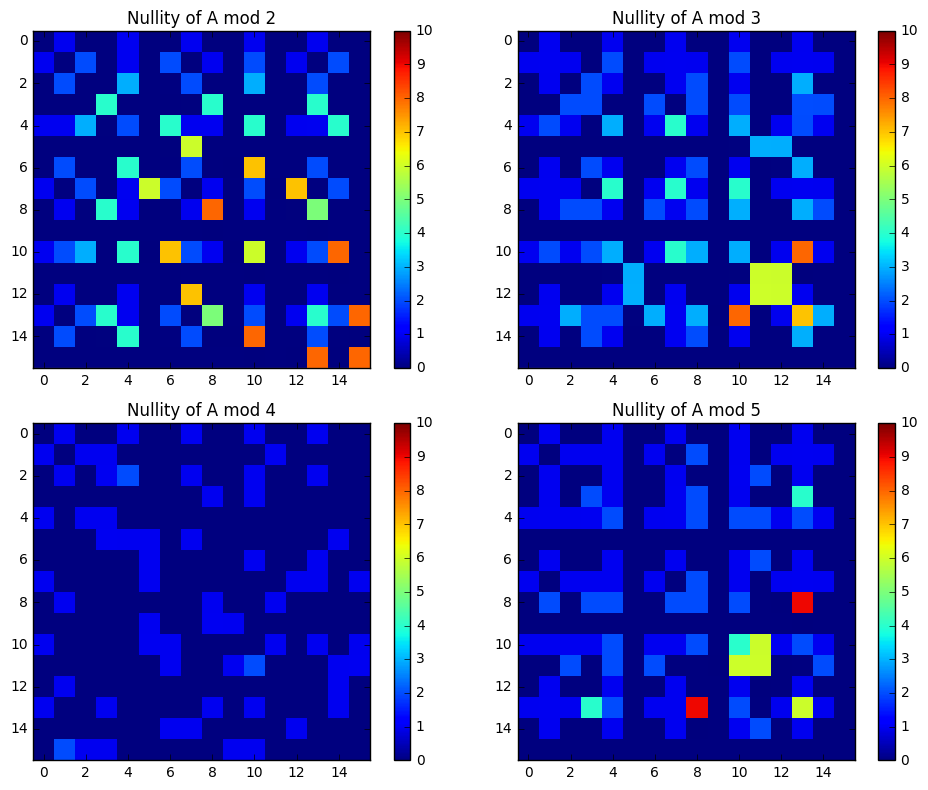
\includegraphics[width=0.67\textwidth]{nullity.png}


\begin{thebibliography}{9}
\bibitem{jaap}
  J. Scherphuis, \textit{The Mathematics of Lights Out},
  \href{http://www.jaapsch.net/puzzles/lomath.htm}{http://www.jaapsch.net/puzzles/lomath.htm}.
  Accessed December 2016.
\bibitem{giffen}
  A. Giffen and D. B. Parker, \textit{On Generalizing the "Lights Out" Game and a Generalization of Parity Domination}, preprint, 2009. Available at \href{http://faculty.gvsu.edu/parkerda/profstuff/papers/hyperlogpd.pdf}{http://faculty.gvsu.edu/parkerda/profstuff/papers/hyperlogpd.pdflink}.
\bibitem{involve}
  S. Edwards, V. Elandt, N. James, K. Johnson, Z. Mitchell, and D. Stephenson, \textit{Lights Out on finite graphs}, Involve 3 (2010), 17-32. Available at \href{http://msp.org/involve/2010/3-1/involve-v3-n1-p03-s.pdf}{http://msp.org/involve/2010/3-1/involve-v3-n1-p03-s.pdf}.
\end{thebibliography}

\end{document}
